%BAB_3 LAPORAN KP

\chapter{PERANCANGAN SISTEM}

\section{Metode Perancangan sistem}
	Perancangan proyek ini diawali dengan menentukan metode yang tepat untuk mendesain dan membangun sistem secara keseluruhan meliputi perancangan Elektronis,Pemrogramman mikrokontroller, perancangan Antar muka, implementasi PID pada kontroller, dan implementasi \textit{invers kinematic} pada Antar muka.
	
	\begin{figure}[H]
		\centering
		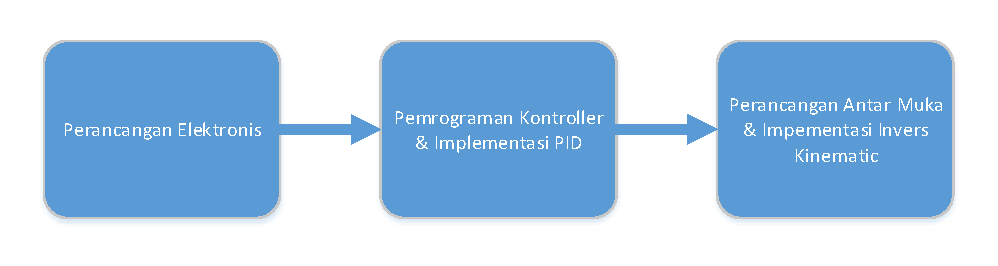
\includegraphics[width=\linewidth]{Visio/diagram_blok.pdf}
		\caption{Diagram metode perancangan sistem}
	\end{figure}
	
	\subsection{Perancangan Elektronis}
	
	\subsection{Pemrograman Kontroller \& Implementasi PID}
	
	\subsection{Perancangan Antar Muka \& Inplementasi \textit{Invers Kinematic}}
	